\section*{Bài tập 04 --- Phân lớp Naive Bayes}

Giả định \textbf{Naive Bayes}: các thuộc tính (đã cho trong từng câu) \textbf{độc lập có điều kiện} theo lớp. Dùng \textbf{Laplace} với tham số \(\alpha=1\): làm trơn \emph{cả} xác suất tiên nghiệm và các xác suất điều kiện của thuộc tính rời rạc; với từ vựng ở Câu~3 làm trơn trên \(V=7\) loại từ.

Khi so sánh hai lớp chỉ cần \(\log\) (hoặc lũy thừa tích); hằng số chung có thể bỏ qua.

%--------------------------------------------------------------------
\subsection*{Câu 1 --- Dữ liệu chơi tennis (toàn rời rạc)}

Có \(14\) mẫu: \(|\text{No}|=5\), \(|\text{Yes}|=9\).

\subsubsection*{(a) Tiên nghiệm và likelihood}

Với \(2\) lớp, làm trơn tiên nghiệm:
\[
P(\text{No})=\frac{5+1}{14+2}=\frac{6}{16}=\frac{3}{8}=0{,}375,\qquad
P(\text{Yes})=\frac{9+1}{16}=\frac{5}{8}=0{,}625.
\]

Với thuộc tính rời rạc có \(V\) giá trị khác nhau trong tập huấn luyện, trong lớp \(c\) có \(n_c\) mẫu:
\[
P(\text{giá trị}=v\mid c)=\frac{\text{số lần }v\text{ xuất hiện trong }c+\alpha}{n_c+\alpha V}.
\]

Đếm trên từng lớp ta có các bảng sau (đã kiểm lại đủ mọi giá trị trong miền của từng cột).

\medskip
\noindent\textbf{Lớp No} (\(n_{\text{No}}=5\)):

\begin{center}
{\small
\begin{tabular}{@{}ll@{}}\toprule
Thuộc tính & \(P(\cdot\mid \text{No})\) sau Laplace \\\midrule
Outlook &
  Sunny \(\frac{3+1}{5+3}=\frac12\); Rainy \(\frac{2+1}{8}=\frac38\); Overcast \(\frac{0+1}{8}=\frac18\). \\
Temp &
  Hot \(\frac{2+1}{5+3}=\frac38\); Mild \(\frac{2+1}{8}=\frac38\); Cool \(\frac{1+1}{8}=\frac14\). \\
Humidity &
  High \(\frac{4+1}{5+2}=\frac57\); Normal \(\frac{1+1}{7}=\frac27\). \\
Windy &
  False \(\frac{2+1}{5+2}=\frac37\); True \(\frac{3+1}{7}=\frac47\). \\
\bottomrule
\end{tabular}
}
\end{center}

\noindent\textbf{Lớp Yes} (\(n_{\text{Yes}}=9\)):

\begin{center}
{\small
\begin{tabular}{@{}ll@{}}\toprule
Thuộc tính & \(P(\cdot\mid \text{Yes})\) sau Laplace \\\midrule
Outlook &
  Sunny \(\frac{2+1}{9+3}=\frac14\); Rainy \(\frac{3+1}{12}=\frac13\); Overcast \(\frac{4+1}{12}=\frac{5}{12}\). \\
Temp &
  Hot \(\frac{2+1}{12}=\frac14\); Mild \(\frac{4+1}{12}=\frac{5}{12}\); Cool \(\frac{3+1}{12}=\frac13\). \\
Humidity &
  High \(\frac{3+1}{9+2}=\frac{4}{11}\); Normal \(\frac{6+1}{11}=\frac{7}{11}\). \\
Windy &
  False \(\frac{6+1}{9+2}=\frac{7}{11}\); True \(\frac{3+1}{11}=\frac{4}{11}\). \\
\bottomrule
\end{tabular}
}
\end{center}

\subsubsection*{(b) Mẫu \texttt{(Sunny, Cool, High, Windy=True)}}

Tính \(\tilde P(c)\propto P(c)\,P(\text{Sunny}\mid c)\,P(\text{Cool}\mid c)\,P(\text{High}\mid c)\,P(\text{True}\mid c)\).

\emph{Lớp No:}
\[
\frac{3}{8}\cdot\frac12\cdot\frac14\cdot\frac57\cdot\frac47
=\frac{3\cdot 5\cdot 4}{8\cdot 2\cdot 4\cdot 7\cdot 7}=\frac{60}{3136}\approx 0{,}0191.
\]

\emph{Lớp Yes:}
\[
\frac{5}{8}\cdot\frac14\cdot\frac13\cdot\frac{4}{11}\cdot\frac{4}{11}
=\frac{5\cdot 4\cdot 4}{8\cdot 4\cdot 3\cdot 11\cdot 11}=\frac{80}{11616}\approx 0{,}00688.
\]

Ta có \(0{,}0191>0{,}0069\) nên \textbf{dự đoán: No} (không chơi).

\subsubsection*{(c) Outlook không quan sát được: \texttt{(?, Cool, High, Windy=True)}}

Do
\[
\sum_{o} P(\text{Outlook}=o\mid c)=1,
\]
khi \textbf{không biết} Outlook, ta \textbf{không nhân} thêm bất kỳ hệ số Outlook nào; chỉ còn
\[
\tilde P(c)\propto P(c)\,P(\text{Cool}\mid c)\,P(\text{High}\mid c)\,P(\text{True}\mid c).
\]

\emph{No:} \(\frac{3}{8}\cdot\frac14\cdot\frac57\cdot\frac47\approx 0{,}0268\).

\emph{Yes:} \(\frac{5}{8}\cdot\frac13\cdot\frac{4}{11}\cdot\frac{4}{11}\approx 0{,}0246\).

Vẫn lớn hơn ở No, nên \textbf{dự đoán: No}.

%--------------------------------------------------------------------
\subsection*{Câu 2 --- Cùng 14 mẫu nhưng nhiệt độ và độ ẩm là số}

Outlook và Windy coi như rời rạc (Laplace như Câu~1). Với Temperature và Humidity, trong mỗi lớp \(c\) ước lượng trung bình \(\mu\) và \textbf{độ lệch chuẩn mẫu} \(s\) (mẫu có cỡ \(n_c>1\), chia \(n_c-1\)):
\[
f(x\mid c)=\frac{1}{\sqrt{2\pi}\,s}\exp\Bigl(-\frac{(x-\mu)^2}{2s^2}\Bigr).
\]

Từ dữ liệu (nhãn \texttt{yes}/\texttt{no} như đề):

\medskip
\noindent\textbf{Tiên nghiệm:} \(P(\text{no})=\frac{3}{8}\), \(P(\text{yes})=\frac{5}{8}\) (cùng công thức \(14\) mẫu, \(\alpha=1\), hai lớp).

\noindent\textbf{Tham số Gaussian:}
lớp \textbf{no} (\(5\) mẫu): \(\mu_T=74{,}6\), \(s_T\approx 7{,}893\); \(\mu_H=84\), \(s_H\approx 9{,}618\).

Lớp \textbf{yes} (\(9\) mẫu): \(\mu_T=73\), \(s_T\approx 6{,}164\); \(\mu_H\approx 78{,}222\), \(s_H\approx 9{,}884\).

\noindent\textbf{Likelihood rời rạc} (Outlook/Windy $|$ lớp) trùng với kiểu đếm Laplace trên bảng chữ thường \texttt{sunny}/\texttt{rain}/\texttt{overcast} và \texttt{true}/\texttt{false}; ví dụ: \(P(\text{sunny}\mid\text{no})=\frac12\), \(P(\text{sunny}\mid\text{yes})=\frac14\), \(P(\text{Windy}=\text{true}\mid\text{no})=\frac47\), \(P(\text{true}\mid\text{yes})=\frac{4}{11}\), \ldots

\begin{figure}[htbp]
  \centering
  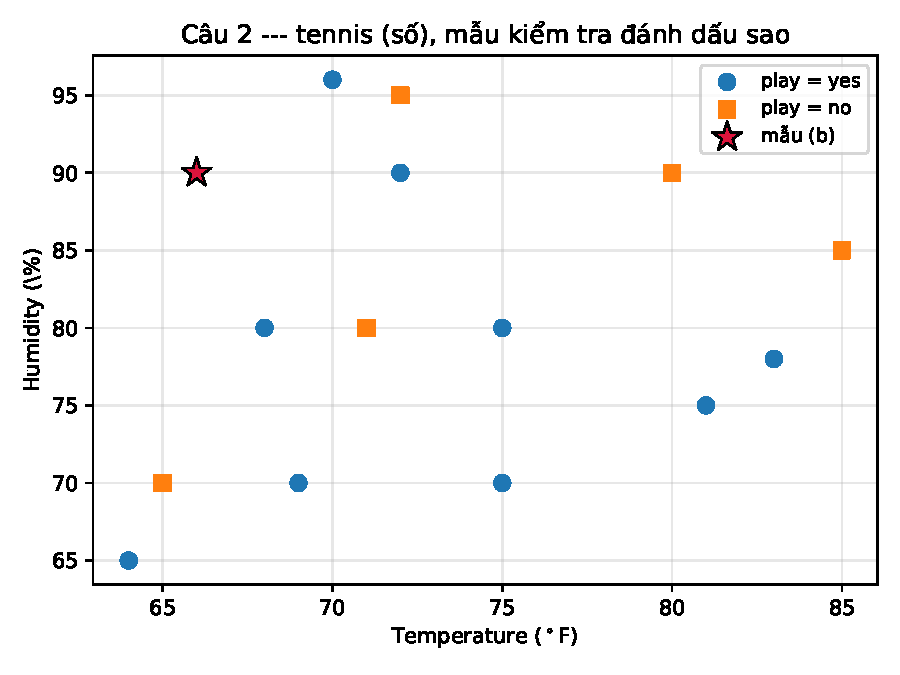
\includegraphics[width=0.72\linewidth]{figures/q2_temp_humidity_scatter.pdf}
  \caption{Câu 2: phân bố điểm huấn luyện theo hai lớp; ngôi sao là mẫu cần phân lớp ở phần~(b).}
\end{figure}

\subsubsection*{(b) Phân lớp mẫu \texttt{(sunny, 66, 90, windy=true)}}

Nhân tiên nghiệm, hai mật độ Gaussian (tại \(T=66\), \(H=90\)) và hai xác suất rời rạc. Tổng \(\log\) hậu nghiệm lớn hơn ở lớp \textbf{no}, nên \textbf{dự đoán: no}.

%--------------------------------------------------------------------
\subsection*{Câu 3 --- Email: Multinomial Naive Bayes}

Huấn luyện: hai thư \textbf{N}, một thư \textbf{S}; tổng \(3\) văn bản.

Tiên nghiệm (hai lớp, \(\alpha=1\)):
\[
P(\text{N})=\frac{2+1}{3+2}=\frac{3}{5},\qquad
P(\text{S})=\frac{1+1}{5}=\frac{2}{5}.
\]

Gộp chỉ số từ trong toàn bộ thư cùng lớp:

\medskip
\noindent\textbf{Lớp N:} tổng số lần xuất hiện từ \(=10\) (từ E1 và E2).

\[P(w_i\mid \text{N})=\frac{\text{đếm}(w_i\text{ trong N})+1}{10+7}=\frac{\text{đếm}+1}{17}.\]

Cụ thể:
\(P(w_1\mid \text{N})=\frac{2}{17}\), \(P(w_2\mid \text{N})=\frac{5}{17}\), \(P(w_3\mid \text{N})=\frac{2}{17}\), \(P(w_4\mid \text{N})=\frac{1}{17}\), \(P(w_5\mid \text{N})=\frac{3}{17}\), \(P(w_6\mid \text{N})=\frac{2}{17}\), \(P(w_7\mid \text{N})=\frac{2}{17}\).

\noindent\textbf{Lớp S:} tổng lần xuất hiện \(=5\) (thư E3).

\[P(w_i\mid \text{S})=\frac{\text{đếm}+1}{5+7}=\frac{\text{đếm}+1}{12}.\]

Cụ thể:
\(P(w_1\mid \text{S})=\frac{2}{12}\), \(P(w_2\mid \text{S})=\frac{1}{12}\), \(P(w_3\mid \text{S})=\frac{2}{12}\), \(P(w_4\mid \text{S})=\frac{2}{12}\), \(P(w_5\mid \text{S})=\frac{1}{12}\), \(P(w_6\mid \text{S})=\frac{3}{12}\), \(P(w_7\mid \text{S})=\frac{1}{12}\).

\subsubsection*{(b) Thư E4 có bộ đếm \((1,0,0,0,0,0,1)\)}

Chỉ \(w_1\) và \(w_7\) có tần suất dương. So sánh
\[
\tilde P(\text{N})\propto P(\text{N})\,P(w_1\mid \text{N})\,P(w_7\mid \text{N})
=\frac{3}{5}\cdot\frac{2}{17}\cdot\frac{2}{17}
\]
và
\[
\tilde P(\text{S})\propto \frac{2}{5}\cdot\frac{2}{12}\cdot\frac{1}{12}.
\]

Ta có \(\frac{3}{5}\cdot\frac{4}{289}\approx 0{,}00830\) và \(\frac{2}{5}\cdot\frac{2}{144}\approx 0{,}00556\), nên \textbf{dự đoán: N} (không spam).
